% ##################################################################################################################
\chapter{Belgium: The Use of MATSim Within an Estimation Framework for Assessing Economic Impacts of River Floods}
\label{ch:belgium}
\hfill \textbf{Author:} Ismaïl Saadi, Jacques Teller, Mario Cools

\editdone{This text has undergone the professional edit. Please no grammatical changes anymore! They are most-probably wrong.}

% ##################################################################################################################
\section{Problem Statement}
With the history of river floods in Belgium and the significant probability that such events will again take place in the near future, assessment of both direct and indirect economic impact was deemed essential to allow formulation of an adequate policy program and efficient flood risk management. 
One proposal would assess flood risk  at the micro-scale level: \ie individual buildings for exposure analysis and direct economic damage estimation, individual companies for indirect economic damage estimation, 10\,meter grid spacing for land-use modeling and individuals/vehicles for transportation models. 
To enable this assessment, an integrated modeling framework combining different simulation theories from a multidisciplinary perspective is being developed. 
Figure~\ref{fig:belgium_fig1} describes the procedure to measure the annual flood risk. 
A more detailed description of the whole modeling chain is available in \citet[][]{DewalsEtAl_IAHR_2015}.

 % ------------
\createfigure%
{Economic impact estimation procedure}%
{Economic impact estimation procedure}%
{\label{fig:belgium_fig1}}%
{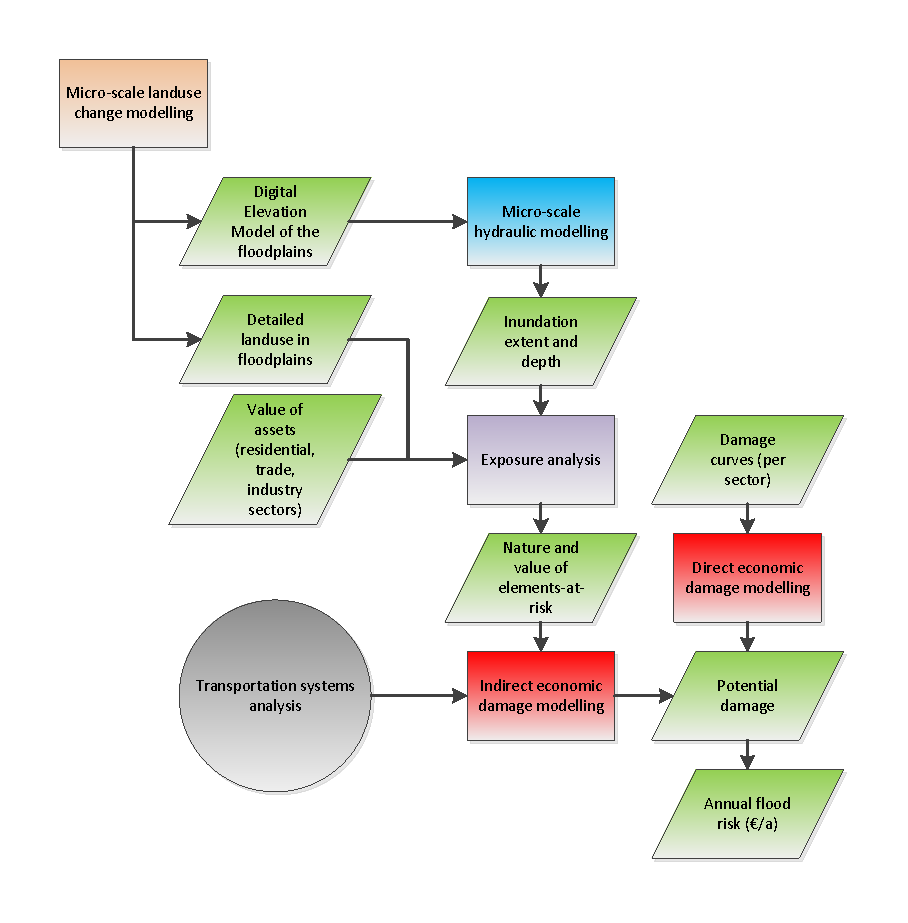
\includegraphics[width=0.97\textwidth, angle=0]{scenarios/figures/belgium_fig1.pdf}}%
{}
% ------------

A basic modeling framework premise is that different spatial pattern 'families' might influence the damage intensity caused by river floods (\eg land use change, transportation systems). 
In this chapter, we focus on how \gls{matsim} is being integrated into this overall framework, thus focusing on the \gls{tsa} within the overall estimation procedure.  For \gls{tsa}, two configurations (freight and passenger model) are distinguished. 
For the passenger model, a \gls{matsim} scenario is developed on a national scale to simulate travel demand at base year 2010 and its evolution during the following years. 
The main objective is to study the effects of river floods on the transportation network and, consequently, on travel demand from an economic point of view. 
In addition, a freight travel demand model has been developed, to enable interactions between passenger and goods flows. 
Note: at this time, this is still an aggregate four-step model, but development is ongoing to develop an agent-based model for the freight side.  

% ##################################################################################################################
\section{Data Collection}
As inputs, \gls{matsim} requires a synthetic population (or travel demand) file, as well as the related transportation network. 
Unfortunately, no recent census is available for the first input; 
the latest dates from~2001. 
To compensate, a synthetic population was derived from more recent travel surveys \citep[e.g.,][]{CornelisEtAl_ResRep_BELDAM_2012} by employing a Gibbs sampler \citep[][]{FarooqBierlaireHurtubiaEtAl2013Simulationbasedpopulation}. 
The Belgian National Household Travel Survey \citep[e.g.,][]{CornelisEtAl_ResRep_BELDAM_2012} contains socio-demographics and activity travel diaries with a detailed description of activity start, end times and durations. 
Activity locations are also available, but at the municipality code level. They are generally accessed by using the new municipalities referencing system: \gls{lau} level~2. 
For the transportation network, \gls{osm} network data has been used.

% ##################################################################################################################
\section{Inputs Preparation}
% ========================================================================================
\subsection{Network}
The network data of Belgium, downloaded in~2015, is available online from the \gls{osm} server. 
It consists of 100\,467 nodes and 232\,715 links. 
Network quality is generally acceptable, according to many \gls{matsim} users, even if manual adjustment is necessary for specific links.

% ========================================================================================
\subsection{Synthetic Population}
Preparation of a synthetic population presents a significant challenge for this case study; 
only micro-data are available to enable population synthesis. 
From these partial views of the actual population, use of a Gibbs sampler enables the joint distribution (re-)construction. 
The outputs seem to be encouraging when comparing computed predictions to the reference dataset. 
Here, we propose testing the methodology by synthesizing some relevant variables for both transportation and urban systems simulations at the household level (see Figure~\ref{fig:belgium_fig2}).

 % ------------
\createfigure%
{Examples of households synthesized attributes}%
{Examples of households synthesized attributes}%
{\label{fig:belgium_fig2}}%
{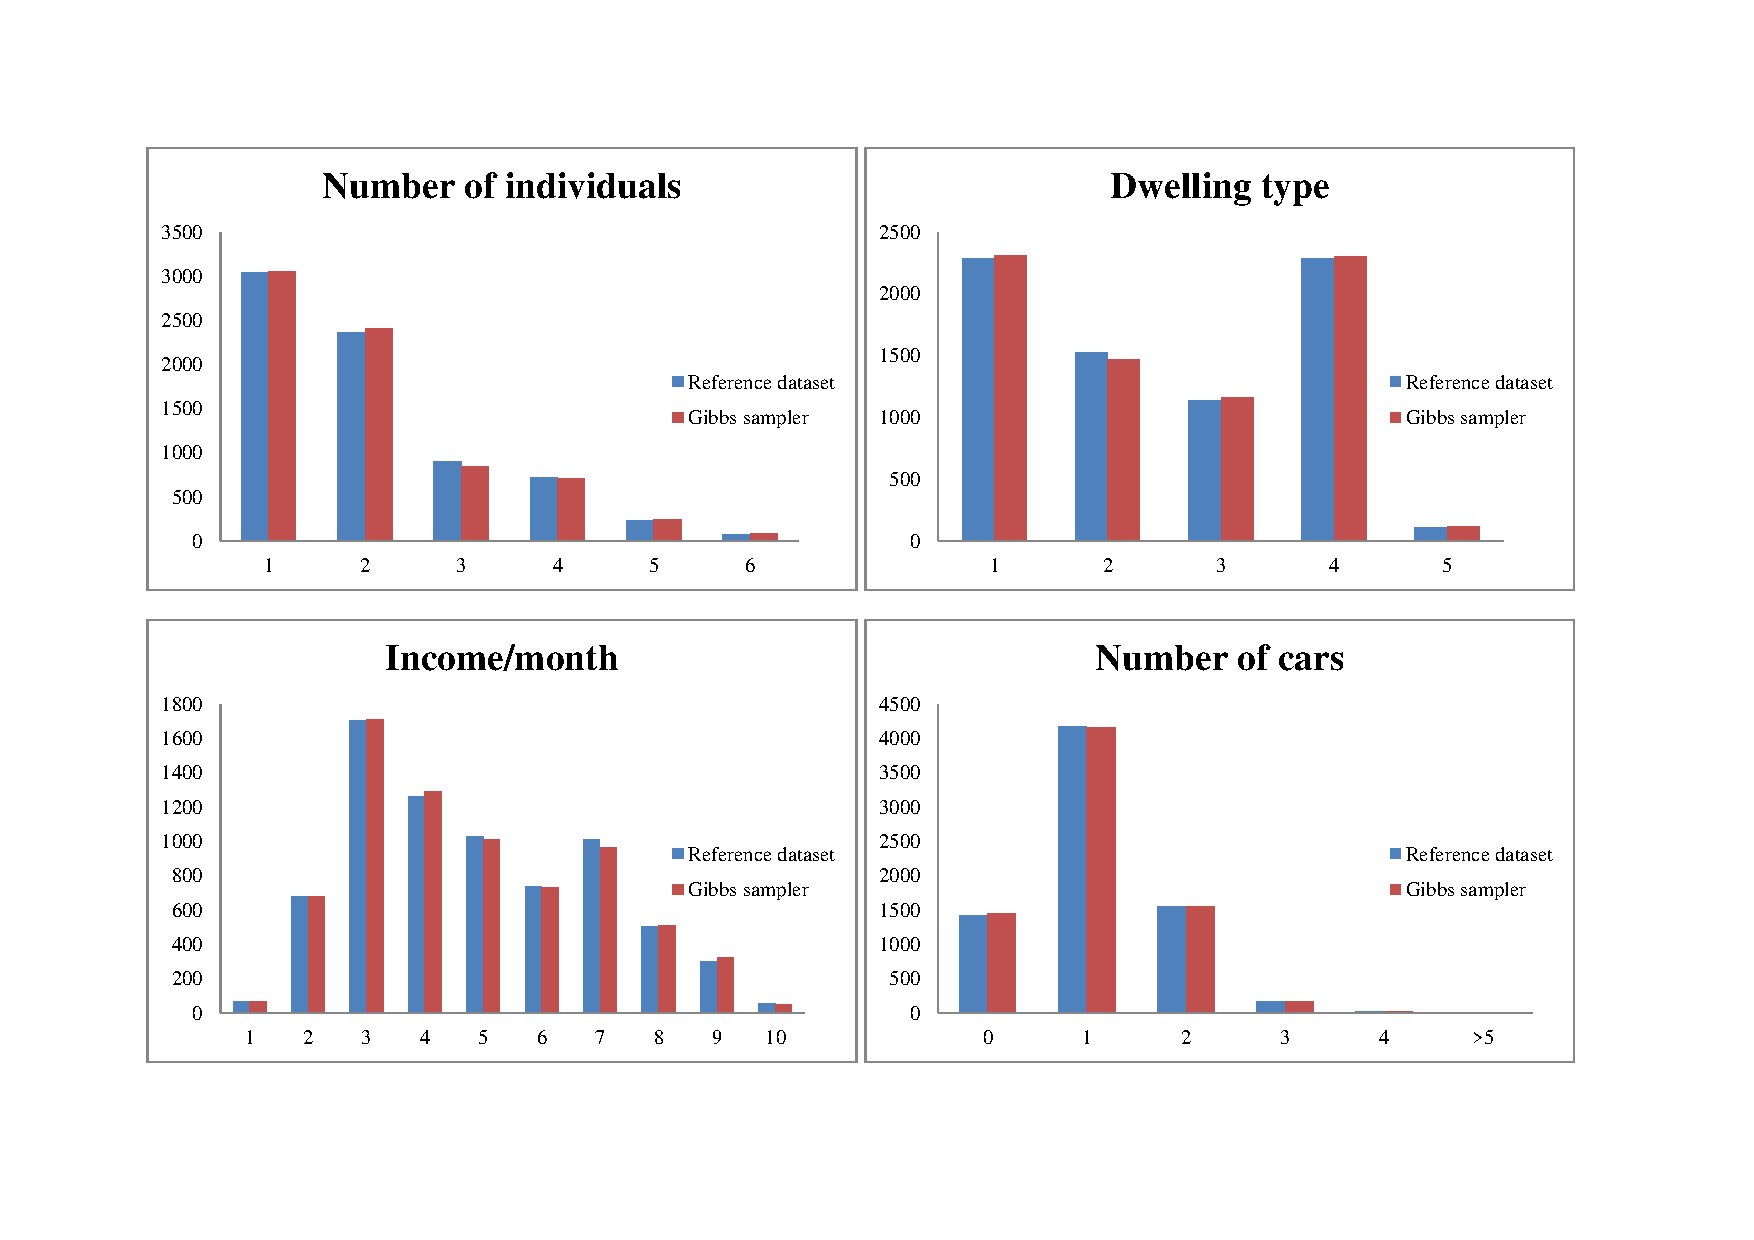
\includegraphics[width=0.97\textwidth, angle=0]{scenarios/figures/belgium_fig2.pdf}}%
{}
% ------------

% ========================================================================================
\subsection{Activity-Based Pattern Generation}
After the synthetic population has been generated, \emph{activity types}, \emph{activity times} and \emph{activity locations} are generated and associated to the agents, using an activity-based pattern generator. 
Using a combined set of machine learning techniques, daily activity planners are generated for each agent. 
As shown in Figure~\ref{fig:belgium_fig3}, the model suggests some promising first results. The activity-pattern generator is calibrated by using micro-data, such as activity travel diaries extracted from travel surveys. 
Calibration quality will be measured after analyzing \gls{matsim} scenario outputs when traffic counts are compared. 
If the comparison between observed and simulated traffic counts suggests a significant deviation, a direct approach based on traffic counts \citep[][]{CoolsEtAl_TRR_2010} could work to adjust activity-based pattern generator parameters.

 % ------------
\createfigure%
{Activity chains generation}%
{Activity chains generation}%
{\label{fig:belgium_fig3}}%
{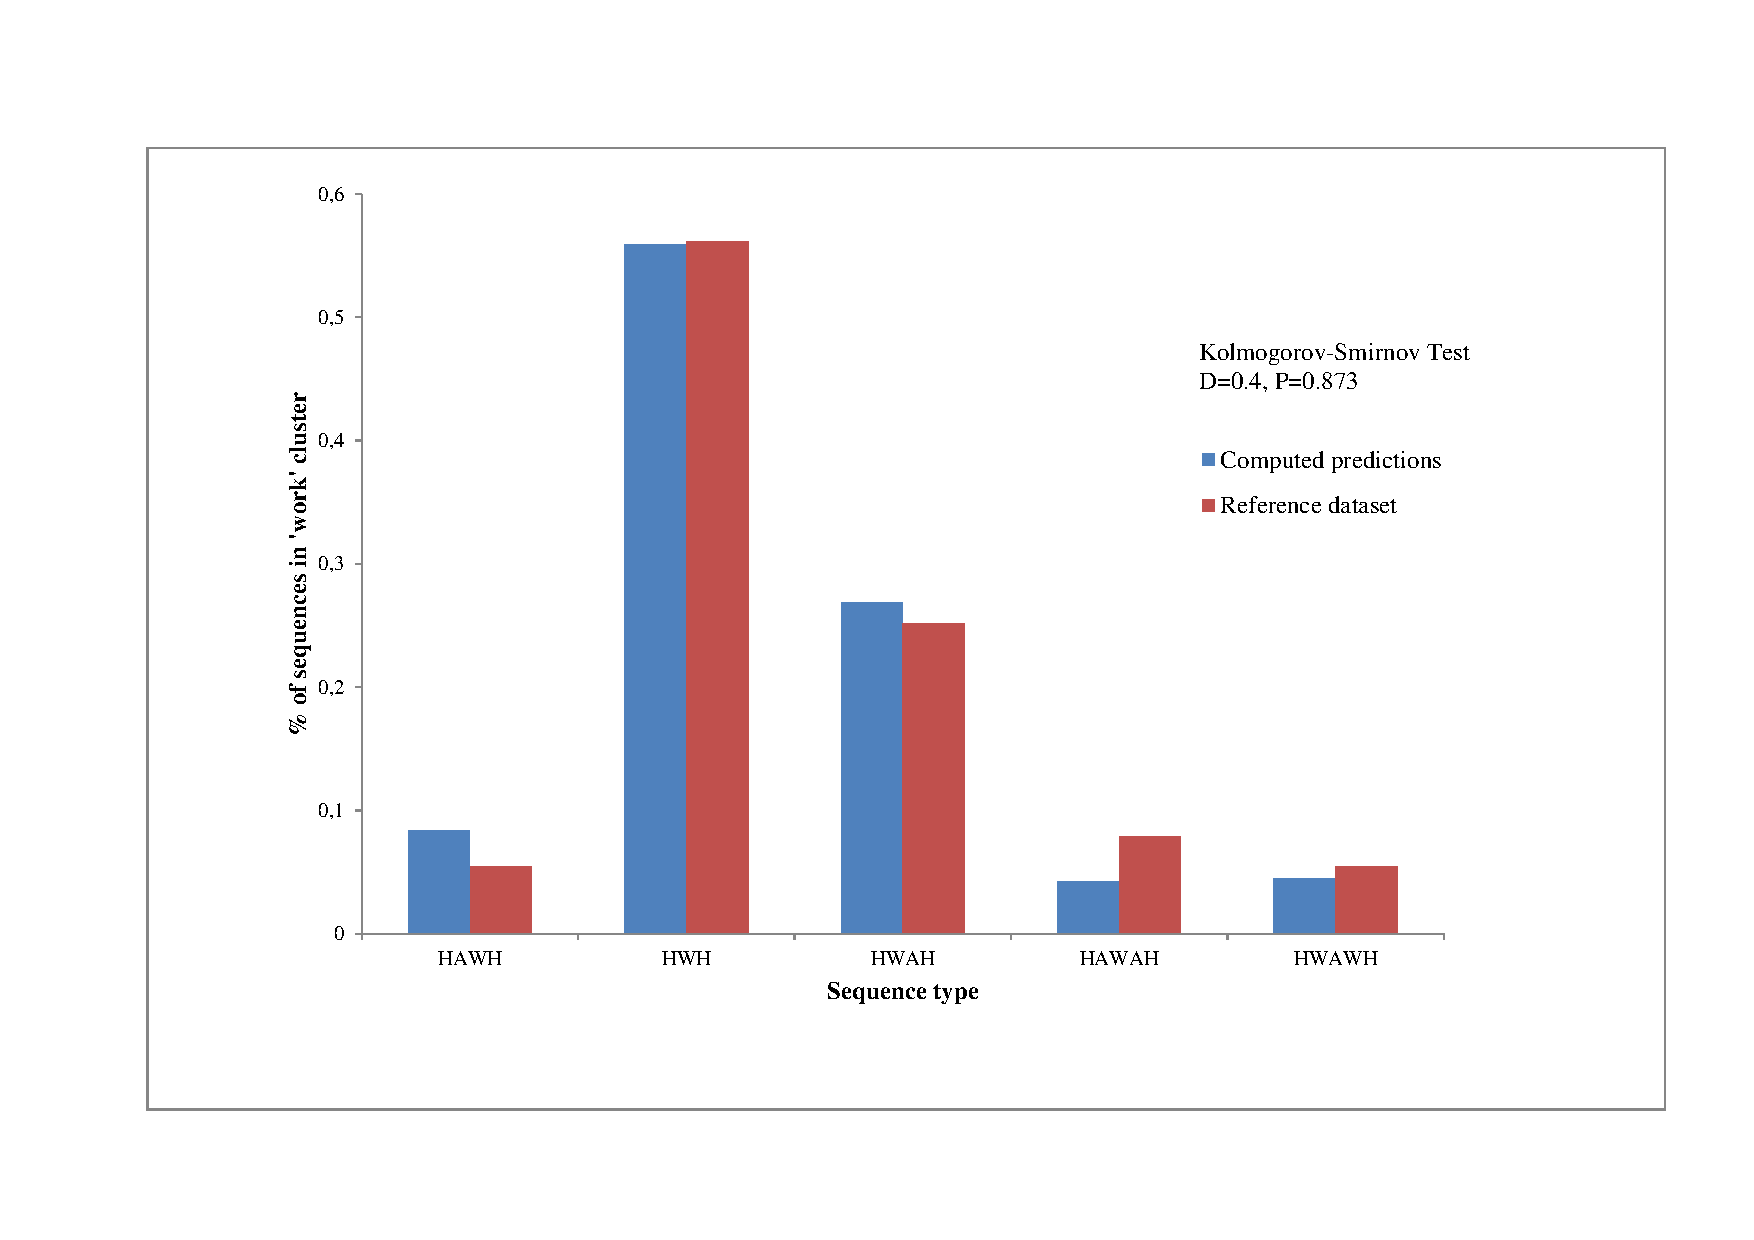
\includegraphics[width=0.97\textwidth, angle=0]{scenarios/figures/belgium_fig3.pdf}}%
{}
% ------------

As outlined by \citet[][]{CoolsEtAl_TRB_2011}, uncertainties introduced by statistical distributions of random components in most activity-based models might be significant. 
Thus, some key indicators (\eg sequences type proportions) will be investigated to measure micro-simulation error impact.

% ##################################################################################################################
\section{General Modeling Framework}
In Saadi et al. (2014), the overall modeling framework is presented, as well as the integration of scheme components. 
This paper covers all concepts expected to be used in building the future \gls{matsim} scenario. 
Figure~\ref{fig:belgium_fig4} is a partial view of the overall modeling framework being researched at the moment.

 % ------------
\createfigure%
{Partial modeling framework}%
{Partial modeling framework}%
{\label{fig:belgium_fig4}}%
{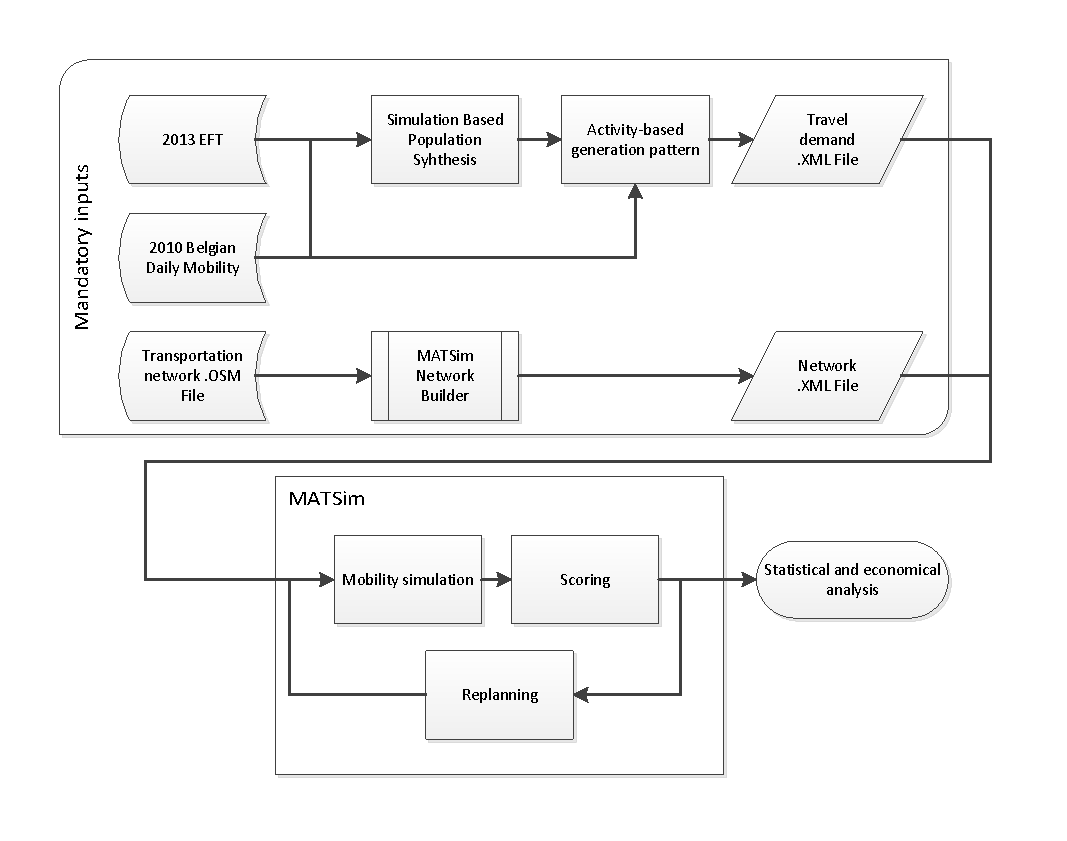
\includegraphics[width=0.97\textwidth, angle=0]{scenarios/figures/belgium_fig4.pdf}}%
{}
% ------------

% ##################################################################################################################
\section{Modeling Network Disruption}
As mentioned, this study also suggests modeling network inaccessibility occurring after river floods. 
This approach assumes that link capacities subjected to river floods are reduced, depending on flood intensity. 
Given that damage is mainly a function of water depth, the idea is to intersect a steady-state inundation map with the transportation network or, at least, the area impacted by floods \citep[][]{SaadiEtAl_ICTTE_2014}. 
Then, an analysis extension will be achieved by including a time series of river floods for a better understanding of dynamic effects: \eg response to river floods propagation, return way and time to the new equilibrium point between transport supply and demand. 
A similar problem was studied in a tsunami evacuation scenario simulation in the city of Padang \citep[][]{LaemmelGretherNagel2009TimeDependentNetworks} (Chapter~\ref{ch:padang}) and was particularly interesting in terms of network dynamic evolution during the scenario simulation.

% ##################################################################################################################
\section{Next Development Steps}
When the complete integrated agent-based transportation model is ready, combination with the land-use change \gls{ca} based model proposed by \citet[][]{MustafaEtAl_PES_2014} will to allow more interactions between those two patterns. 
This connection will be the basis for an innovative micro-scale \gls{luti} model, allowing
more accurate predictions about future river floods influenced by different micro-scale patterns.

% ##################################################################################################################







